% Options for packages loaded elsewhere
\PassOptionsToPackage{unicode}{hyperref}
\PassOptionsToPackage{hyphens}{url}
\PassOptionsToPackage{dvipsnames,svgnames,x11names}{xcolor}
%
\documentclass[
  number]{elsarticle}

\usepackage{amsmath,amssymb}
\usepackage{iftex}
\ifPDFTeX
  \usepackage[T1]{fontenc}
  \usepackage[utf8]{inputenc}
  \usepackage{textcomp} % provide euro and other symbols
\else % if luatex or xetex
  \usepackage{unicode-math}
  \defaultfontfeatures{Scale=MatchLowercase}
  \defaultfontfeatures[\rmfamily]{Ligatures=TeX,Scale=1}
\fi
\usepackage{lmodern}
\ifPDFTeX\else  
    % xetex/luatex font selection
\fi
% Use upquote if available, for straight quotes in verbatim environments
\IfFileExists{upquote.sty}{\usepackage{upquote}}{}
\IfFileExists{microtype.sty}{% use microtype if available
  \usepackage[]{microtype}
  \UseMicrotypeSet[protrusion]{basicmath} % disable protrusion for tt fonts
}{}
\makeatletter
\@ifundefined{KOMAClassName}{% if non-KOMA class
  \IfFileExists{parskip.sty}{%
    \usepackage{parskip}
  }{% else
    \setlength{\parindent}{0pt}
    \setlength{\parskip}{6pt plus 2pt minus 1pt}}
}{% if KOMA class
  \KOMAoptions{parskip=half}}
\makeatother
\usepackage{xcolor}
\setlength{\emergencystretch}{3em} % prevent overfull lines
\setcounter{secnumdepth}{5}
% Make \paragraph and \subparagraph free-standing
\makeatletter
\ifx\paragraph\undefined\else
  \let\oldparagraph\paragraph
  \renewcommand{\paragraph}{
    \@ifstar
      \xxxParagraphStar
      \xxxParagraphNoStar
  }
  \newcommand{\xxxParagraphStar}[1]{\oldparagraph*{#1}\mbox{}}
  \newcommand{\xxxParagraphNoStar}[1]{\oldparagraph{#1}\mbox{}}
\fi
\ifx\subparagraph\undefined\else
  \let\oldsubparagraph\subparagraph
  \renewcommand{\subparagraph}{
    \@ifstar
      \xxxSubParagraphStar
      \xxxSubParagraphNoStar
  }
  \newcommand{\xxxSubParagraphStar}[1]{\oldsubparagraph*{#1}\mbox{}}
  \newcommand{\xxxSubParagraphNoStar}[1]{\oldsubparagraph{#1}\mbox{}}
\fi
\makeatother


\providecommand{\tightlist}{%
  \setlength{\itemsep}{0pt}\setlength{\parskip}{0pt}}\usepackage{longtable,booktabs,array}
\usepackage{calc} % for calculating minipage widths
% Correct order of tables after \paragraph or \subparagraph
\usepackage{etoolbox}
\makeatletter
\patchcmd\longtable{\par}{\if@noskipsec\mbox{}\fi\par}{}{}
\makeatother
% Allow footnotes in longtable head/foot
\IfFileExists{footnotehyper.sty}{\usepackage{footnotehyper}}{\usepackage{footnote}}
\makesavenoteenv{longtable}
\usepackage{graphicx}
\makeatletter
\def\maxwidth{\ifdim\Gin@nat@width>\linewidth\linewidth\else\Gin@nat@width\fi}
\def\maxheight{\ifdim\Gin@nat@height>\textheight\textheight\else\Gin@nat@height\fi}
\makeatother
% Scale images if necessary, so that they will not overflow the page
% margins by default, and it is still possible to overwrite the defaults
% using explicit options in \includegraphics[width, height, ...]{}
\setkeys{Gin}{width=\maxwidth,height=\maxheight,keepaspectratio}
% Set default figure placement to htbp
\makeatletter
\def\fps@figure{htbp}
\makeatother

\makeatletter
\@ifpackageloaded{caption}{}{\usepackage{caption}}
\AtBeginDocument{%
\ifdefined\contentsname
  \renewcommand*\contentsname{Table of contents}
\else
  \newcommand\contentsname{Table of contents}
\fi
\ifdefined\listfigurename
  \renewcommand*\listfigurename{List of Figures}
\else
  \newcommand\listfigurename{List of Figures}
\fi
\ifdefined\listtablename
  \renewcommand*\listtablename{List of Tables}
\else
  \newcommand\listtablename{List of Tables}
\fi
\ifdefined\figurename
  \renewcommand*\figurename{Figure}
\else
  \newcommand\figurename{Figure}
\fi
\ifdefined\tablename
  \renewcommand*\tablename{Table}
\else
  \newcommand\tablename{Table}
\fi
}
\@ifpackageloaded{float}{}{\usepackage{float}}
\floatstyle{ruled}
\@ifundefined{c@chapter}{\newfloat{codelisting}{h}{lop}}{\newfloat{codelisting}{h}{lop}[chapter]}
\floatname{codelisting}{Listing}
\newcommand*\listoflistings{\listof{codelisting}{List of Listings}}
\makeatother
\makeatletter
\makeatother
\makeatletter
\@ifpackageloaded{caption}{}{\usepackage{caption}}
\@ifpackageloaded{subcaption}{}{\usepackage{subcaption}}
\makeatother

\ifLuaTeX
  \usepackage{selnolig}  % disable illegal ligatures
\fi
\usepackage[]{natbib}
\bibliographystyle{elsarticle-num}
\usepackage{bookmark}

\IfFileExists{xurl.sty}{\usepackage{xurl}}{} % add URL line breaks if available
\urlstyle{same} % disable monospaced font for URLs
\hypersetup{
  pdftitle={Draft -- Effect of Atmospheric Heatwaves on Reflectance and Pigment Composition of Intertidal Nanozostera noltei -- Draft},
  pdfauthor={Simon Oiry; Bede Ffinian Rowe Davies; Philippe Rosa; Augustin Debly; Maria Laura Zoffoli; Anne-Laure Barillé; Nicolas Harin; Pierre Gernez; Laurent Barillé},
  pdfkeywords={Remote Sensing, Pigment Composition, Seagrass, Coastal
Ecosystems, Heatwaves},
  colorlinks=true,
  linkcolor={blue},
  filecolor={Maroon},
  citecolor={Blue},
  urlcolor={Blue},
  pdfcreator={LaTeX via pandoc}}


\setlength{\parindent}{6pt}
\begin{document}

\begin{frontmatter}
\title{Draft -- Effect of Atmospheric Heatwaves on Reflectance and
Pigment Composition of Intertidal \emph{Nanozostera noltei} -- Draft}
\author[1]{Simon Oiry%
\corref{cor1}%
}
 \ead{oirysimon@gmail.com} 
\author[1]{Bede Ffinian Rowe Davies%
%
}

\author[1]{Philippe Rosa%
%
}

\author[1]{Augustin Debly%
%
}

\author[2]{Maria Laura Zoffoli%
%
}

\author[3]{Anne-Laure Barillé%
%
}

\author[3]{Nicolas Harin%
%
}

\author[1]{Pierre Gernez%
%
}

\author[1]{Laurent Barillé%
%
}


\affiliation[1]{organization={Institut des Substances et Organismes de
la Mer, ISOMer, Nantes Université, UR 2160, F-44000 Nantes,
France},,postcodesep={}}
\affiliation[2]{organization={Consiglio Nazionale delle Ricerche,
Istituto di Scienze Marine (CNR-ISMAR), 00133 Rome,
Italy},,postcodesep={}}
\affiliation[3]{organization={Bio-littoral, Immeuble Le Nevada, 2 Rue du
Château de l'Eraudière, 44300 Nantes, France},,postcodesep={}}

\cortext[cor1]{Corresponding author}









        
\begin{abstract}
To be written
\end{abstract}





\begin{keyword}
    Remote Sensing \sep Pigment Composition \sep Seagrass \sep Coastal
Ecosystems \sep 
    Heatwaves
\end{keyword}
\end{frontmatter}
    

\section{Introduction}\label{introduction}

Intertidal seagrasses play a crucial role in the ecosystem by providing
habitats and feeding grounds for various marine species, supporting rich
marine biodiversity, and contributing significantly to primary
production and carbon sequestration
\citep{unsworth2022planetary, sousa2019blue}. These seagrasses are
essential in maintaining the health of coastal ecosystems by stabilizing
sediments, filtering water, and serving as indicators of environmental
changes due to their sensitivity to water quality variations
\citep{zoffoli2021decadal}. The interactions between seagrass meadows
and their associated herbivores further enhance the delivery of
ecosystem services, including coastal protection and fisheries support
\citep{jankowska2019stabilizing, zoffoli2023remote, gardner2018global}.
Understanding and preserving these ecosystems are vital for maintaining
the biodiversity and productivity of coastal regions
\citep{scott2018role, ramesh2020seagrass}.

Despite their crucial role in marine ecosystems, intertidal seagrasses
face numerous threats that compromise their health and functionality.
Coastal development and human activities are primary threats. These
activities not only reduce the available habitat for seagrasses but also
increase water turbidity, which limits light penetration and hampers
photosynthesis \citep{waycott2009accelerating}. Seagrasses are also
threatened by nutrient enrichment from agricultural and urban runoff,
which can lead to eutrophication. This condition promotes the overgrowth
of algal blooms that compete with seagrasses for light and nutrients,
further stressing these important plants \citep{thomsen2023meadow} (Oiry
et al.~2024). Pollution from industrial and agricultural fields sources
introduces harmful chemicals and heavy metals into coastal waters,
posing toxic risks to seagrass health. These pollutants can affect the
physiological processes of seagrasses, reducing their growth and
survival rates \citep{sevgi2022bitkilerde} Additionally, invasive
species can out compete native seagrasses for resources, altering
community structure and function \citep{simpson2016distribution}.

Heatwaves, exacerbated by climate change, pose a growing threat to
seagrasses. Marine Heatwaves (MHW), defined by
\citep{hobday2016hierarchical} as prolonged discrete anomalously warm
water events, and Atmospheric Heatwaves (AHW), defined by
\citep{perkins2013measurement} as periods of at least three consecutive
days with temperatures exceeding the 90th percentile, cause severe
physiological stress on seagrasses
\citep{sawall2021chronically, deguette2022physiological}. At the
interface between the land and oceans, intertidal seagrasses are exposed
to both MHW and AHW. Heatwaves have profound impacts on seagrasses, with
their effects varying based on species and geographic location. For
instance, the seagrass \emph{Zostera marina} exhibits high
susceptibility to elevated sea surface temperatures during winter and
spring, leading to advanced flowering, high mortality rates, and reduced
biomass \citep{sawall2021chronically}. Similarly, \emph{Cymodocea
nodosa} shows increased photosynthetic activity during heatwaves but
suffers negative effects on photosynthetic performance and leaf biomass
during recovery \citep{deguette2022physiological}. Additionally,
different populations of \emph{Zostera marina} along the European
thermal gradient exhibit varied photophysiological responses during the
recovery phase of heatwaves, indicating differential adaptation
capabilities among populations \citep{winters2011effects}. These events
intensify other stressors, such as overgrazing and seed burial,
compromising sexual recruitment \citep{guerrero2020heat}.

Remote sensing is increasingly being used to monitor marine ecosystems,
including seagrass meadows. Spectral indices such as the Normalized
Difference Vegetation Index (NDVI) and the Soil-Adjusted Vegetation
Index (SAVI) are effective for quantifying vegetation health over time
\citep{huete2012vegetation, kloos2021agricultural, carlan2020identifying, akbar2020mangrove}.
By analyzing specific spectral patterns, remote sensing can track
changes in seagrass meadows with high temporal and spatial resolution.
Europe promotes these techniques through frameworks like the Water
Framework Directive and the Marine Strategy Framework Directive, which
advocate for habitat mapping using remote sensing technologies to cover
large areas and detect long-term trends
\citep{papathanasopoulou2019satellite}.

This study aims to experimentally test the hypothesis that warm events,
such as atmospheric heatwaves, alter the pigment composition and
reflectance of the intertidal seagrass Nanozostera noltei. By linking
these changes with satellite remote sensing data, the study seeks to
provide insights into how heatwaves affect seagrass meadows and to
assess the potential of remote sensing in monitoring these impacts

\section{Material \& Methods}\label{material-methods}

\subsection{Observation of seagrass leaves
darkening.}\label{observation-of-seagrass-leaves-darkening.}

\subsubsection{Field Observation}\label{field-observation}

\phantomsection\label{cell-fig-quiberonMap}
\begin{figure}[H]

\centering{

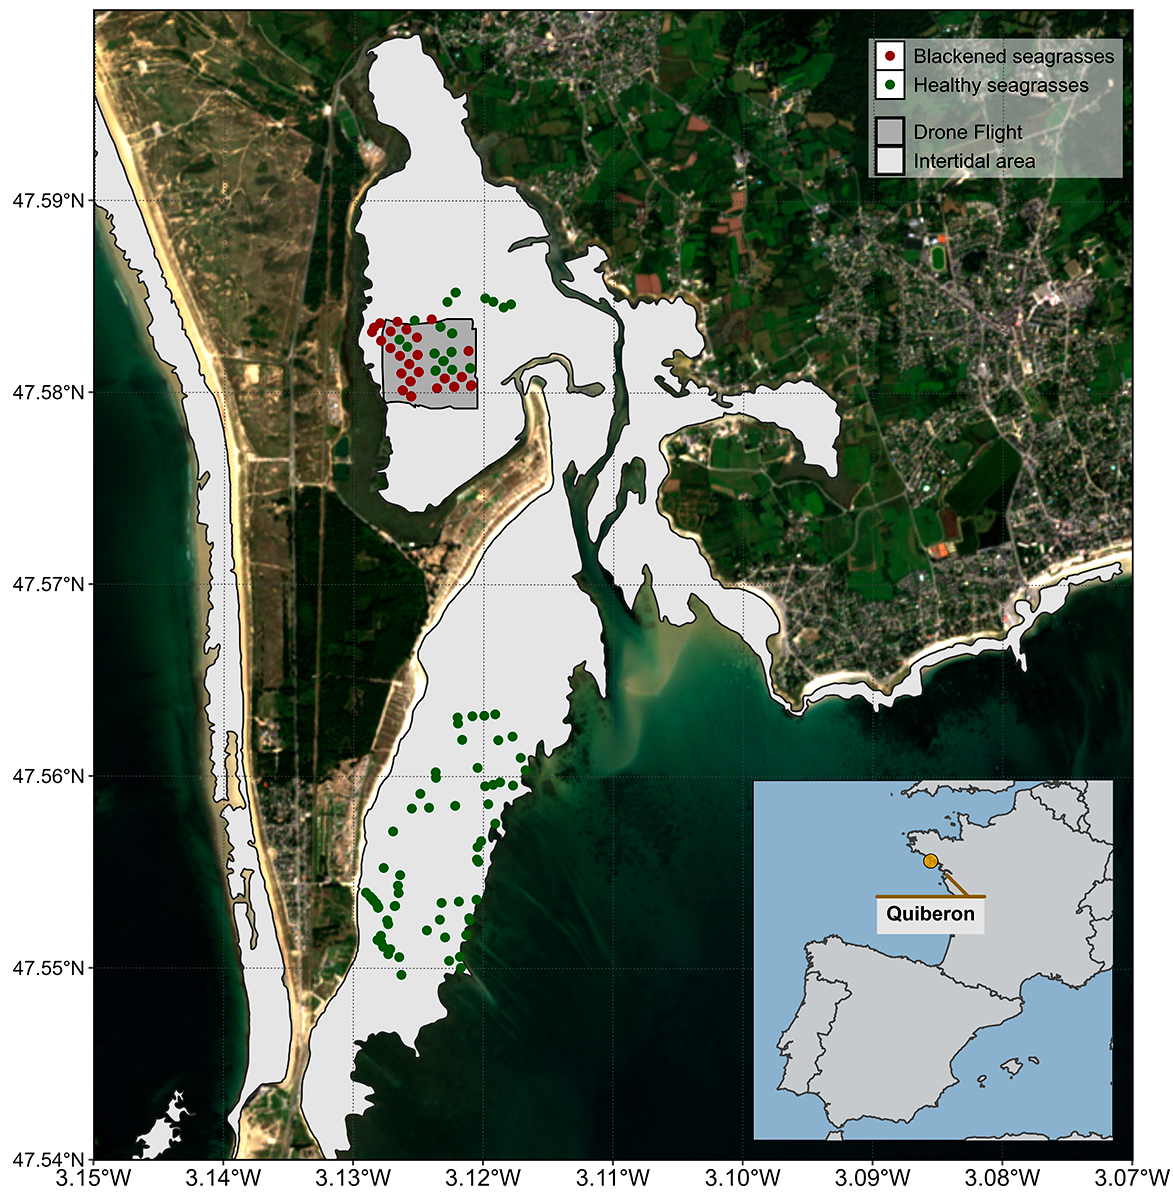
\includegraphics[width=1\textwidth,height=\textheight]{Figs/Low_res/Quiberon_map.png}

}

\caption{\label{fig-quiberonMap}Location of the fieldtrip campaign that
occured in the 10th of September 2021. The light grey polygons indicates
the intertidal zone (Zone between High tide and low tide, that is
totally emerged at low tide) and the dark grey polygon indicate the
extent of the drone flight. Green dots indicate location of quadrat
picture over green seagrasses while red dots indicate location of
quadrat took over darkened seagrasses.}

\end{figure}%

A fieldtrip, aiming to map a seagrass meadow near Quiberon (France :
46°57'32.0''N, 2°10'37.0''W), occurred in the 10th of September 2021
(Figure~\ref{fig-quiberonMap}). During this fieldtrip, darkening of
seagrasses have been observed, resulting in the darkening of seagrass
leaves over large area of the meadow (Figure~\ref{fig-QuiberonImg} C \&
D). During this field trip, drone flights were conducted over two areas
of the seagrass meadow using a DJI Matrice 200 equipped with a Sequoia
Multispectral camera. The Sequoia captures four spectral bands: Green
(550 ± 40 nm), Red (660 ± 40 nm), RedEdge (735 ± 10 nm), and Near
Infrared (790 ± 40 nm). A total of 122 Ground Control Points (GCPs) were
collected in the form of georeferenced quadrat images across the meadow
. These images allow for visual assessment of vegetation type, density,
and health status. The images were then divided into two categories:
green seagrasses and darkened seagrasses, based on a visual estimation
of the leaf condition (Figure~\ref{fig-quiberonMap}).

\phantomsection\label{cell-fig-QuiberonImg}
\begin{figure}[H]

\centering{

\includegraphics[width=1\textwidth,height=\textheight]{Figs/Low_res/img_Quiberon.png}

}

\caption{\label{fig-QuiberonImg}Illustrations of the two health
conditions of seagrasses observed in the field. A: Global view of a
green green meadow; B: Quadrat images of green seagrasses; C: Quadrat
images of darkened seagrasses; D: Global view of an darkened meadow. All
images were taken on September 10th, 2021, in Quiberon.}

\end{figure}%

\subsubsection{Temparature Data and identification of
heatwaves}\label{temparature-data-and-identification-of-heatwaves}

\paragraph{Air temperature}\label{air-temperature}

Since January 1, 2024, Meteo France weather data has been freely and
openly accessible. Hourly air temperature data (°C) for the French
Atlantic and Channel coasts was retrieved using a
\href{https://github.com/SigOiry/HeatWave_Seagrasses/blob/main/Scripts/MeteoFrance_Extraction.qmd}{custom
script} as no API was available at the time of this study. Weather
stations located within 10 kilometers of the coastline were considered,
but only those with at least 30 years of data were included to ensure
reliable climatological reconstruction. Of the 156 weather stations
within 10 kilometers of the coast, only 36 had sufficient data for
climatology reconstruction. The hourly data was then aggregated into
daily mean temperatures for each station.

Heatwave detection was performed using the HeatwaveR package in R
\citep{heatwaveR}. This package utilizes the methodology proposed by
\citep{hobday2016hierarchical} to detect heatwave events. The
climatology for the year was computed using the temperature time series.
An event was considered a heatwave each time the temperature exceeded
the 90th percentile of the climatology for three consecutive days. The
severity of each event has been assessed using the methodology proposed
by \citep{hobday2018categorizing}. Following the methodology of
\citep{schlegel2017nearshore}, coldspell events corresponding to
temperature bellow the percentile 10th of the climatology during 3
consecutives days have also been measured.

Concerning heatwaves event near Quiberon, this methodology has been
apply solely on the nearest weather station of our study site
(Lorient-Lann Bihoue, 47°45'46''N 3°26'11''W , more than 395000
observation since the 1st of February 1952).

\paragraph{Water temperature}\label{water-temperature}

SST data from the Copernicus CMEMS platform were downloaded for the
French coast near Quiberon (47°29′03″N, 3°07′09″W), covering 1982-2022
\citep{CMEMS_1}. Only pixels within an area of 2700 km² around Quiberon,
Brittany, France (47°29′03″N, 3°07′09″W) were extracted and analyzed.
This area was large enough to minimize missing values caused by cloud
cover, yet small enough to avoid being influenced by the stability of
offshore SST. The multi-sensor Level 3S Sea Surface Temperature (SST)
product the we used is built from nighttime infrared satellite data,
including sources like ESA SST CCI, C3S, and EUMETSAT. Data from AVHRR,
ATSR, and SLSTR radiometers are used, but only those with a quality
level above 4. An intercalibration method ensures consistency, and a
daily reference SST field is constructed by combining the best data with
median values from other sources. A large-scale bias correction is
applied, and daily single-sensor composites are merged into a
multi-sensor file (L3S), selecting the best sensor for each grid cell. A
daily average was computed for the time series, and the HeatwaveR
package \citep{heatwaveR} was used to compute SST climatology and detect
SST events using the same method as air temperature event detection.

\subsubsection{Satellite Observation}\label{satellite-observation}

Two Sentinel-2 images covering the field trip site
(Figure~\ref{fig-quiberonMap}) were downloaded from the Copernicus
platform \citep{copernicus_sentinel2}. The first image was taken before
the heatwave event on September 1, 2021, and the second one after the
event on September 6, 2021. Both images were acquired at Level-2
processing, in surface reflectance, and were orthorectified and
atmospherically corrected to account for the effects of the atmosphere
on reflectance values \citep{sen2cor}.

Reflectance value of each GCPs (Figure~\ref{fig-quiberonMap}) have been
exctracted and compared before and after the heatwave event.

\subsubsection{Emersion Time of
Seagrasses}\label{emersion-time-of-seagrasses}

To estimate the emersion time of seagrasses during low tide, both
bathymetric and tidal data are required.

\paragraph{Bathymetry}\label{bathymetry}

Bathymetry data for the study site were obtained from the ``Service
Hydrographique et Océanographique de la Marine''
\citep{shom_bathymetry_litto3d_bzh_2018_2021}. The reference ``zero'' of
this product is based on the NGF/IGN69, which refers to the mean sea
level recorded at the Marseille tide gauge between 1885 and 1897. This
reference is known as the Terrestrial Altimetric Zero.

\paragraph{Tides}\label{tides}

Tidal data for the heatwave events at the study site were downloaded
from the Intergovernmental Oceanographic Commission data portal
\citep{ioc_sea_level_lecy}, for the nearest tide gauge located at Le
Conquet. The ``zero'' for this dataset corresponds to the lowest
astronomical tide, also known as the Hydrographic Zero.

\paragraph{Reference intercalibration of both
dataset}\label{reference-intercalibration-of-both-dataset}

Since the altitude references of these two datasets differ, a correction
factor must be applied to adjust the reference of one dataset to match
the other. The SHOM annually provides a document called ``Références
Altimétriques Marines'' \citep[RAM,][]{shom_ram_2022}, which includes
correction factors for each seaport along the French coastline. These
factors allow, among other things, the conversion of the Terrestrial
Altimetric Zero to the Hydrographic Zero. For Le Conquet, the correction
factor is 2.850 meters.

\subsection{Laboratory experiment}\label{laboratory-experiment}

\subsubsection{Sampling and acclimation of
seagrasses}\label{sampling-and-acclimation-of-seagrasses}

Seagrass was sampled from a \emph{Nanozostera noltei} (dwarf eelgrass,
syn. \emph{Zostera noltei}) meadow on Noirmoutier Island, France
(46°57'32.0''N, 2°10'37.0''W) at low tide in June 2024. A home-made inox
sampling box was used to sample seagrass from an area of 30 cm by 15 cm
and 5 cm deep, maintaining the sediment structure and avoiding damage to
the rhizomes and the leafs of the seagrass (Figure~\ref{fig-design} A).
This sampling box allowed to limitate sampling variability between
replicates. The entire system, including seagrass, sediment, meiofauna,
and macrofauna, was placed in plastic trays together in a mesocosm
setup, which allowed for the natural interactions between components to
be maintained and reduced stress on the seagrass. To avoid hydric stress
during transportation, seawater was added to each tray. Simultaneously,
seawater was sampled from a nearby site and transported to the lab,
where it was filtered using a 0.22 µm nitrocellulose filter to remove
all suspended particulate matter. This seawater was used in the
acclimation tank and the intertidal chambers. The seagrasses were
acclimated at high tide for one weeks with a water temperature of 17°C,
matching the temperature at the time of sampling, and with light of 150
µmol.s-1.m-2 of PAR photons \citep{akbar2020mangrove}. A wave generator
was used in the tank to circulate and reoxygenate the water.

\subsubsection{Experimental design}\label{experimental-design}

\phantomsection\label{cell-fig-design}
\begin{figure}[H]

\centering{

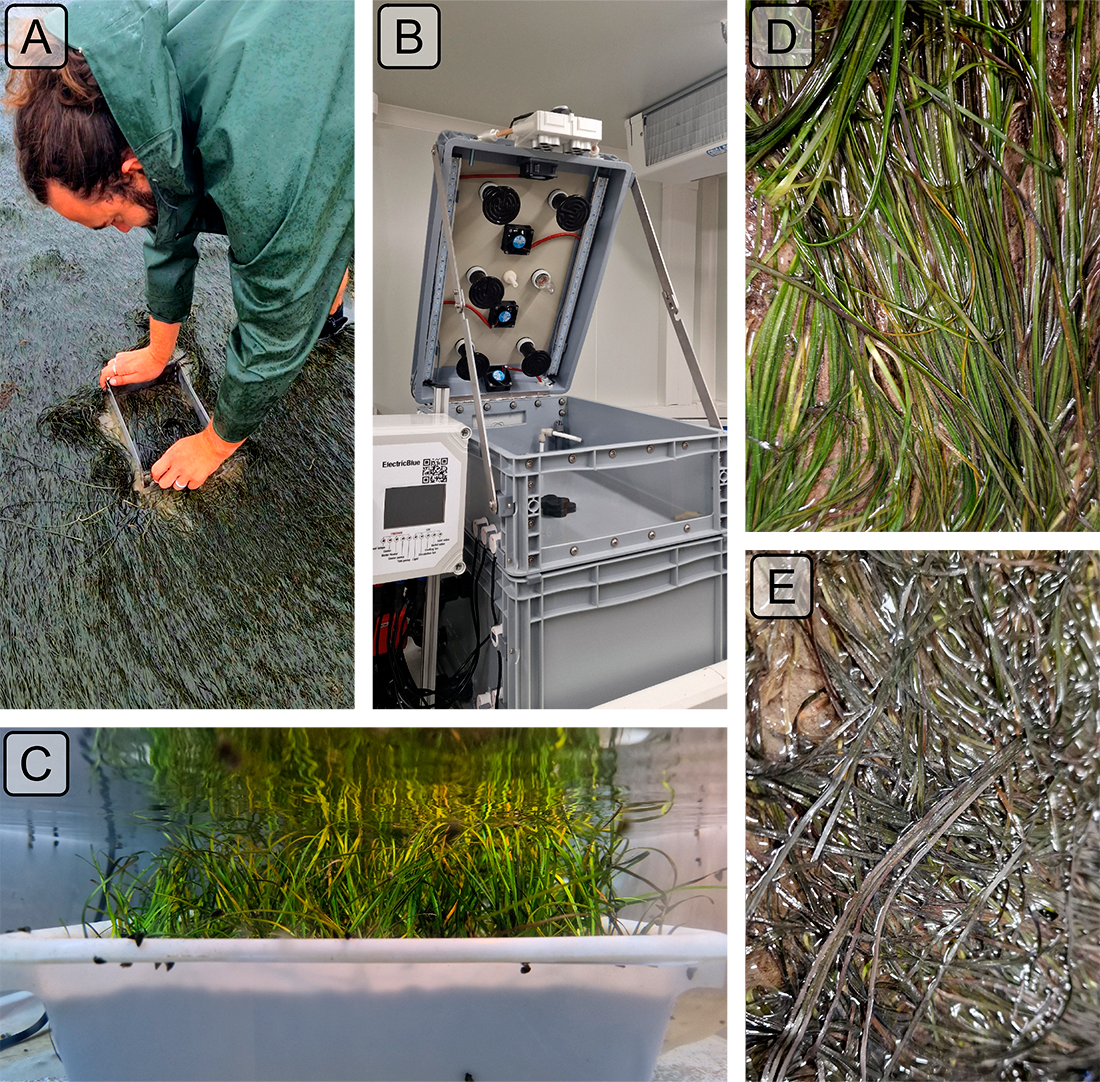
\includegraphics[width=1\textwidth,height=\textheight]{Figs/Low_res/Experimental_design.png}

}

\caption{\label{fig-design}Illustrations of the various steps of the
experiment. A: Field sampling of seagrass using a homemade sampling box;
B: Intertidal chambers used during the experiment; C: Seagrass sample
inside a chamber during the experiment at high tide; D: Photo of the
treatment sample at the start of the experiment; E: Photo of the
treatment sample at the end of the experiment.}

\end{figure}%

Two intertidal chambers from
\href{https://electricblue.eu/intertidal-chamber}{ElectricBlue} were
used to simulate tidal cycles and control water temperature during high
tide and air temperature during low tide (Figure~\ref{fig-design} B,C).
One chamber served as the control, while the other was used for the
experimental treatment.

\phantomsection\label{cell-fig-Temperature_Bourgneuf}
\begin{figure}[H]

\centering{

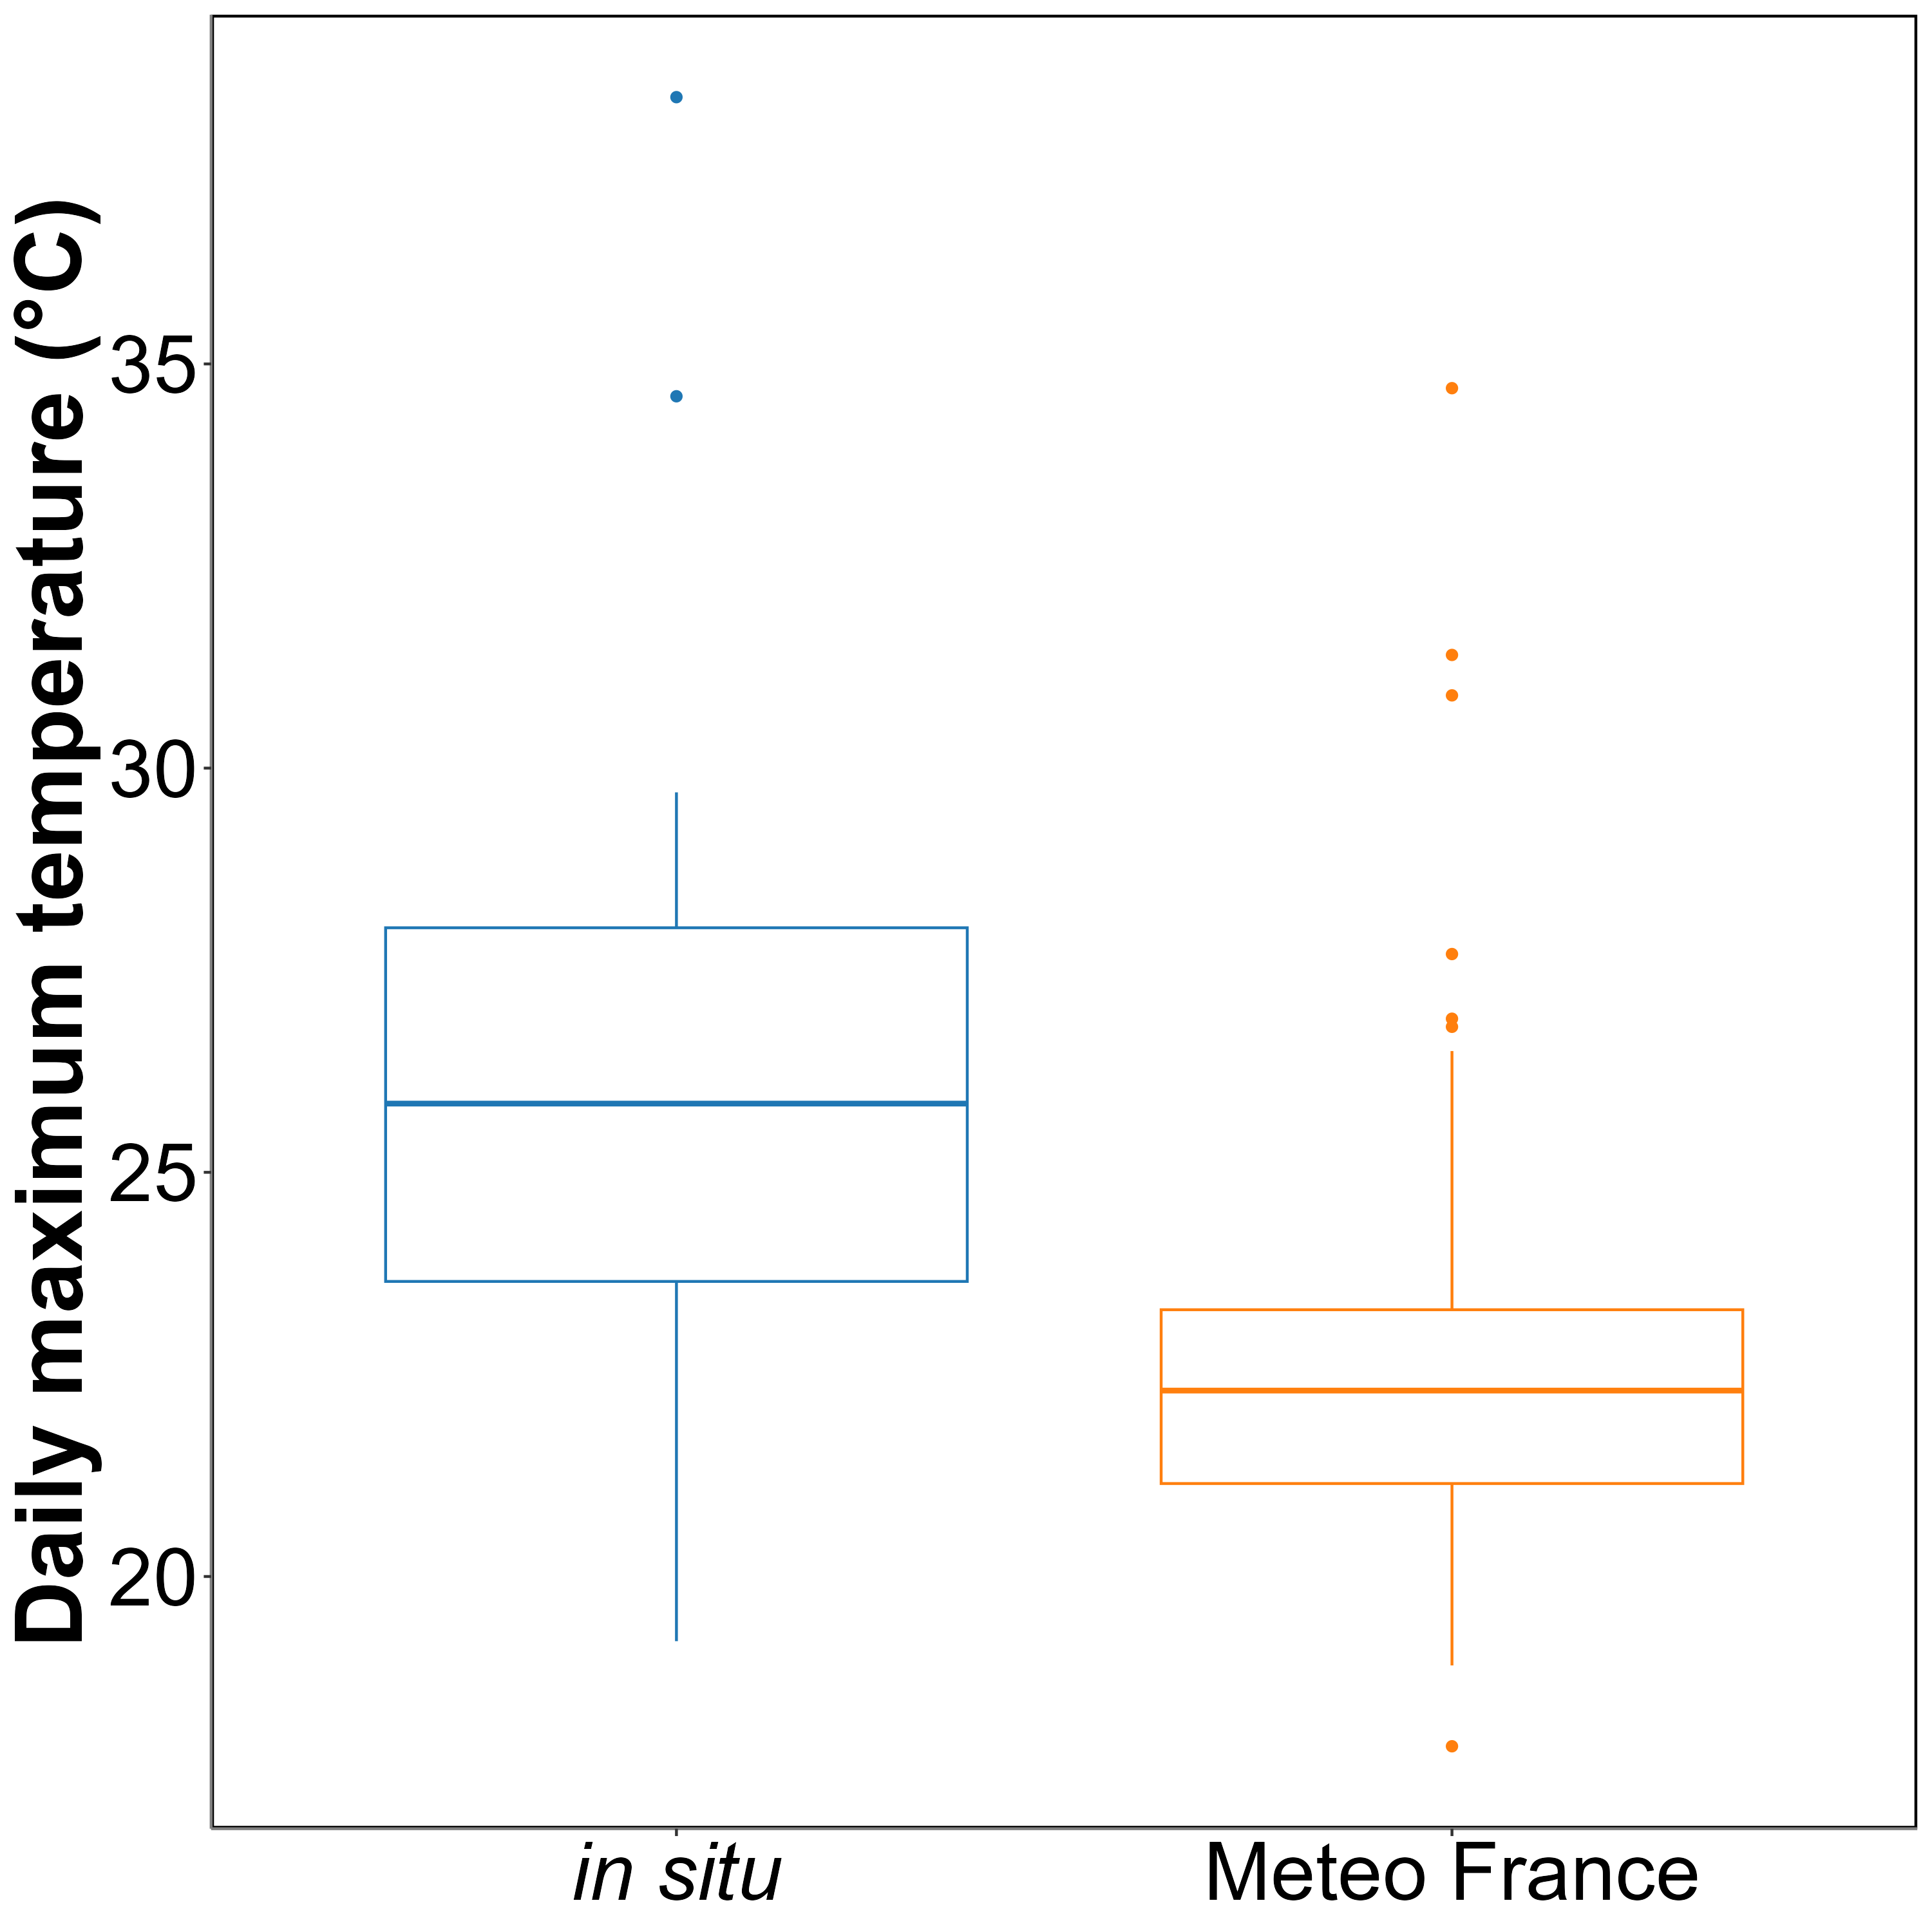
\includegraphics[width=0.3\textwidth,height=\textheight]{Figs/High_res/Temperature_compare.png}

}

\caption{\label{fig-Temperature_Bourgneuf}Comparison of daily maximum
temperatures in August measured using an in-situ sensor (blue) and
retrieved from Meteo France (orange). The solid line in the middle of
the boxplot represents the median, the two ends of the box represent the
25th and 75th percentiles, and the whiskers represent values that are no
more than 1.5 times the interquartile range.}

\end{figure}%

To experimentally apply temperatures that closely mimic those
experienced by seagrasses in the field, \emph{in situ} temperature
sensors were placed at the sampling site in Bourgneuf Bay during August
2024. The daily maximum temperatures recorded by the \emph{in situ}
sensors were compared to those measured by the nearest weather station
operated by Meteo France (Figure~\ref{fig-Temperature_Bourgneuf}). On
average, \emph{in situ} temperatures were 3 ± 3.2°C higher than those
recorded by Meteo France. Additionally, Meteo France temperatures were
more stable compared to those from the \emph{in situ} sensor. This
stability is explained by the fact that Meteo France temperatures are
measured in a sheltered, shaded location . This offset was used to
adjust heatwave temperatures measured by Meteo France to reflect the
conditions experienced by the seagrasses.

The control chamber was maintained at temperatures representative of the
typical seasonal conditions: water temperatures between 18°C and 19°C
and air temperatures between 18°C and 23°C, following circadian
temperature variability (Figure~\ref{fig-Profile} left). For the
experimental treatment, the air temperature was set to mimic an
atmospheric heatwave that occurred over the seagrass meadow of Quiberon,
France (47°35'40.0''N, 3°07'30.0''W) from September 2, 2021, to
September 6, 2021. On the first day of the experiment, air temperatures
in the experimental chamber were set to range from 23°C at night to 35°C
during the day, with a daily increase of 1°C. The water temperature in
the experimental chamber was similarly adjusted to reflect the heatwave
conditions, starting from the normal seasonal range (18°C) and gradually
increasing to simulate the rising temperatures experienced during the
heatwave (+0.5°C daily). This setup aimed to replicate the thermal
stress experienced by the seagrass meadow during the actual heatwave
event (Figure~\ref{fig-Profile} right). The experiment stops only when
no changes in the reflectance of the treatment are observed for 2
consecutive days.

\phantomsection\label{cell-fig-Profile}
\begin{figure}[H]

\centering{

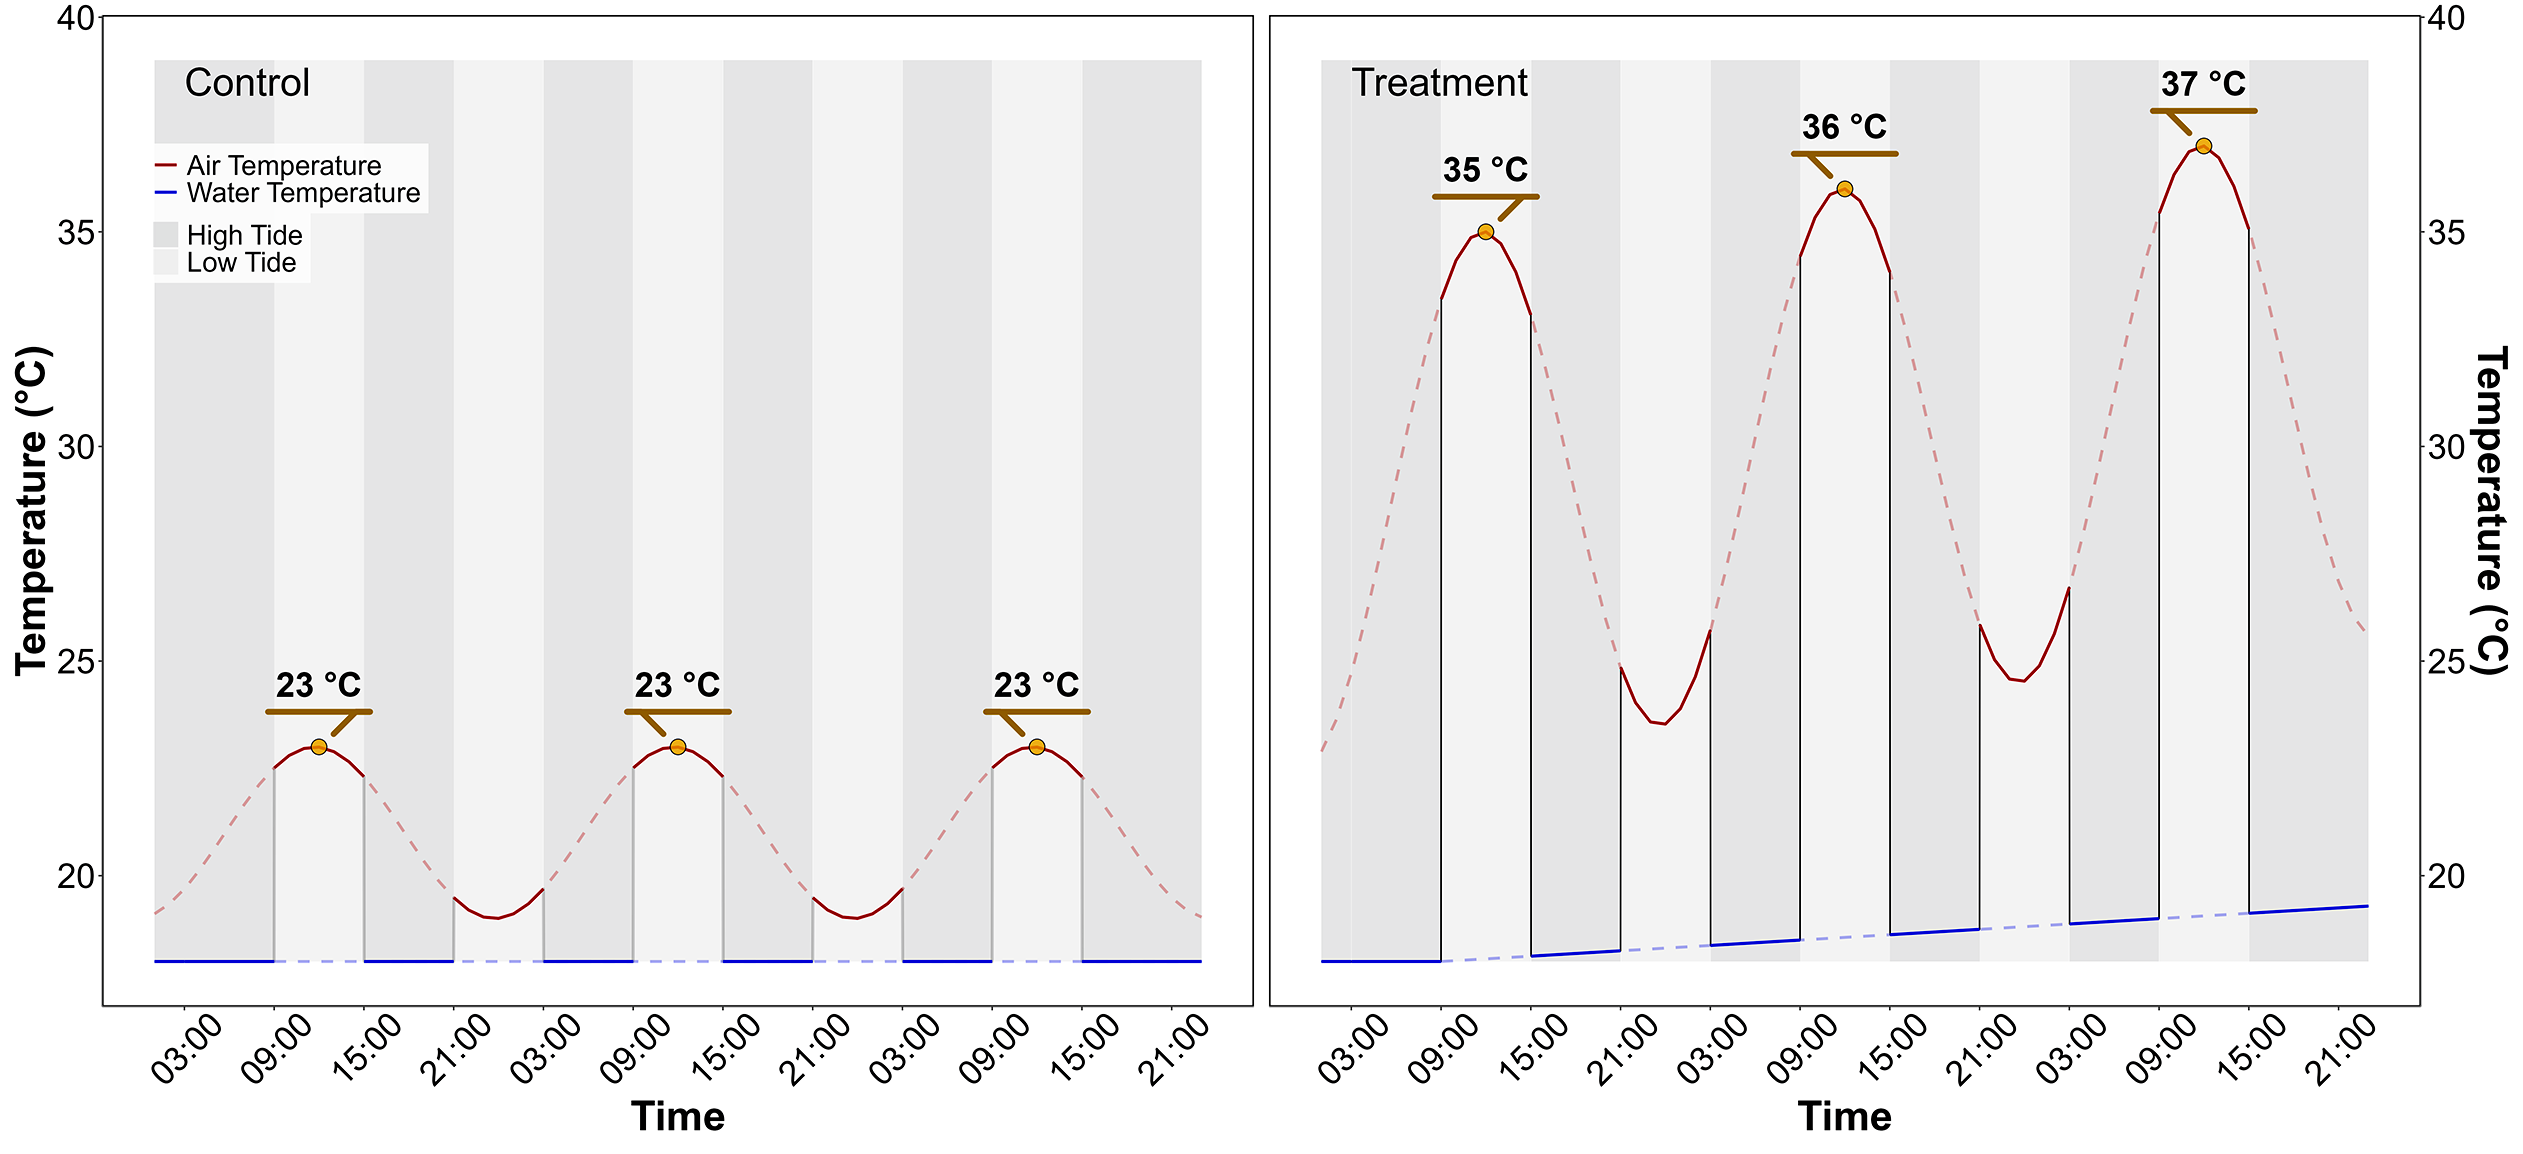
\includegraphics[width=1\textwidth,height=\textheight]{Figs/Low_res/Chamber_Profils.png}

}

\caption{\label{fig-Profile}Temperature profiles of both the control
(left) and the treatment (right) followed during the heatwave
experiment. The red line indicates air temperature, whereas the blue
line indicates water temperature. Due to the tidal cycle followed during
the experiment, the seagrasses only experience temperatures representade
by solid lines.}

\end{figure}%

\subsubsection{Bio-optical measurmenents over seagrass
leaves}\label{bio-optical-measurmenents-over-seagrass-leaves}

\paragraph{Hyperspectral measurements}\label{hyperspectral-measurements}

Throughout the experiment, hyperspectral signatures of both the control
and treatment seagrasses were taken using an ASD HandHeld 2 equipped
with a fiber optic, allowing measurements to be taken directly inside
the chamber without opening it. Automatic spectra acquisition has been
done using the
\href{https://www.malvernpanalytical.com/en/learn/knowledge-center/user-manuals/rs3-software-user-manual}{RS3
softaware} developed by the intrument manufacturer. An average of five
reflectance spectrum (\(R(\lambda)\)), each with an integration time of
544 ms, was taken every minute. Every 10 minutes, the fiber optic was
switched from one benthic chamber to the other, in order to measure
reflectance in both treatment and control. Because light conditions were
controlled inside of the chambers, reflectance calibration of the
instrument was performed only each morning at the very first moment of
low tide using a Spectralon white reference with 99\% Lambertian
reflectivity.

The second derivative of \(R\) was calculated to retrieve absorption
features and compare their variability over time. Two radiometric
indices were also monitored throughout the experiment :

\begin{itemize}
\tightlist
\item
  The Normalized Difference Vegetation Index (NDVI,
  \citep{rouse1974monitoring}), as a proxy of the concentration of
  chlorophyll-a (Equation~\ref{eq-ndvi})
\end{itemize}

\begin{equation}\phantomsection\label{eq-ndvi}{
NDVI = \frac{R(840)-R(668)}{R(840)+R(668)}
}\end{equation}

where \(R(840)\) and \(R(668)\) are the reflectance at 840 nm and 668 nm
respectively.

\begin{itemize}
\tightlist
\item
  The Seagrass Percent Covers, developed by \citep{zoffoli2020sentinel},
  used to assess proportion of seagrass inside of a pixel
  (Equation~\ref{eq-spc}):
\end{itemize}

\begin{equation}\phantomsection\label{eq-spc}{
SPC = 172.06 \times NDVI - 22.18
}\end{equation}

\begin{itemize}
\tightlist
\item
  The Green Leaf Index (GLI, \citep{louhaichi2001spatially}), as a
  measurement of the greenness of seagrass leafs (Equation~\ref{eq-gli})
\end{itemize}

\begin{equation}\phantomsection\label{eq-gli}{
GLI = \frac{[R(550)-R(668)]+[R(550)-R(450)]}{(2 \times R(550) )+ R(668) + R(450) }
}\end{equation}

where \(R(550)\) and \(R(450)\) are the reflectance in green at 550 nm
and in the blue at 450 nm, respectively.

\begin{itemize}
\tightlist
\item
  The Mid-Infrared Water Absorption Index (MIWAI), proposed here and
  designed to measure water absorption at 970 nm (\textbf{REF}),
  estimates the difference between the reflectance at 970 nm and a
  linear interpolation of the reflectance values at 950 and 990 nm. This
  interpolation represents the expected reflectance value in the absence
  of water.
\end{itemize}

\begin{equation}\phantomsection\label{eq-MIWAI}{
MIWAI = 0.5 \times [R(990)+R(950)]-R(970)
}\end{equation}

where \(R(990)\), \(R(970)\) and \(R(950)\) are the reflectance in the
infrared at 990, 970 and 950 nm, respectively.

\begin{quote}
\mbox{}%
\paragraph{Multispectral imagery
measurement}\label{multispectral-imagery-measurement}

Parallel to hyperspectral measurements, multispectral images were taken
at the beginning and end of each diurnal low tide (09:00 am and 03:00
pm). A Micasense RedEdge-MX Dual multispectral camera, originally
designed to be mounted on a drone, was modified for use without a drone.
A 3D-printed mount was designed to attach the camera to the intertidal
chamber and ensure that each picture was captured under the same
conditions. At each time step (09:00 am and 03:00 pm), a first picture
of the Spectralon was taken to allow for image correction in
reflectance, followed by a second picture of the target.
\href{https://sigoiry.github.io/DISCOV-MicaSense/}{DISCOV}, a Neural
Network classification model previously developed to map intertidal
vegetation using drone imagery, has been applied to each image taken
inside the intertidal chambers. To understand the behavior of the model
on seagrasses affected by heatwaves, classification images from before
and after the heatwave have been compared.
\end{quote}

\paragraph{Pigment concentration
measurements}\label{pigment-concentration-measurements}

At the beginning and the end of each diurnal low tide (09:00 am and
03:00 pm) leaves samples have been took in both the test and the
control. leaves sampled have been stored under -80°C waiting for
analysis. Before pigment extraction, each sample was lyophilized and its
dry weight was measured. Pigment composition and biomass were analyzed
using high-performance liquid chromatography (HPLC). The HPLC system
(Alliance HPLC 248 System, Waters) was equipped with a reverse-phase
C-18 separating column (SunFire C-18 Column, 100Å, 3.5 µm, 2.1 mm x 50
mm, Waters), preceded by a precolumn (VanGuard 3.9 mm x 5 mm, Waters).
The system also included a photodiode array detector (2998 PDA) and a
fluorimeter (Ex: 425 nm, Em: 655 nm; RF-20A, SH

\textbf{Au secours Philippe !!!}

\section{Results}\label{results}

\subsection{Heatwaves of Quiberon}\label{heatwaves-of-quiberon}

\subsubsection{Spectral inspection}\label{spectral-inspection}

The Sentinel-2 images used in this study are dated from the 1st of
September 2021 and the 6th of September 2021
(Figure~\ref{fig-S2_comparison} A and C, respectively). The Atmospheric
Heat Wave (AHW) started on 4 September and lasted until 7 September,
while the Marine Heat Wave (MHW) started on 3 September and ended on 8
September 2021 (Figure~\ref{fig-S2_comparison} B). The AHW has been
classified as a strong event, and the MHW has been classified as
moderate. Even though the Sentinel-2 of the 6th of September was
captured only a few days after the start of the events, darkening of
seagrass can already be observed in the true-color composition
(Figure~\ref{fig-S2_comparison} C). Before the event, all GCPs appeared
green un the images, with similar reflectance spectra, regardless of the
class attributed to the GCPs on the field
(Figure~\ref{fig-S2_comparison} A and D left). Their reflectance spectra
showed a peak at 560 nm (in the green part of the spectra), low values
at 665 nm, corresponding to the strong absorption by chlorophyll-a and a
high infrared plateau (\textgreater{} 705 nm). However, GCPs classified
as dark seagrass during the fieldtrip, showed significant differences in
reflectance spectral shape compared to GCPs classified as green seagrass
on the 10th of September, with corresponding differences in the true
color composition (Figure~\ref{fig-S2_comparison} C and D right). In
fact these dark seagrass GCPs were affected by extreme events, which
altered their color and impacted the satellite reflectance
(Figure~\ref{fig-S2_comparison} C). The reflectance spectra over dark
seagrass were characterized by the loss of the reflectance peak at 560
nm and a decrease in the infared plateau, which was observed as a steady
increasing slope up to 940 nm.

\phantomsection\label{cell-fig-S2_comparison}
\begin{figure}[H]

\centering{

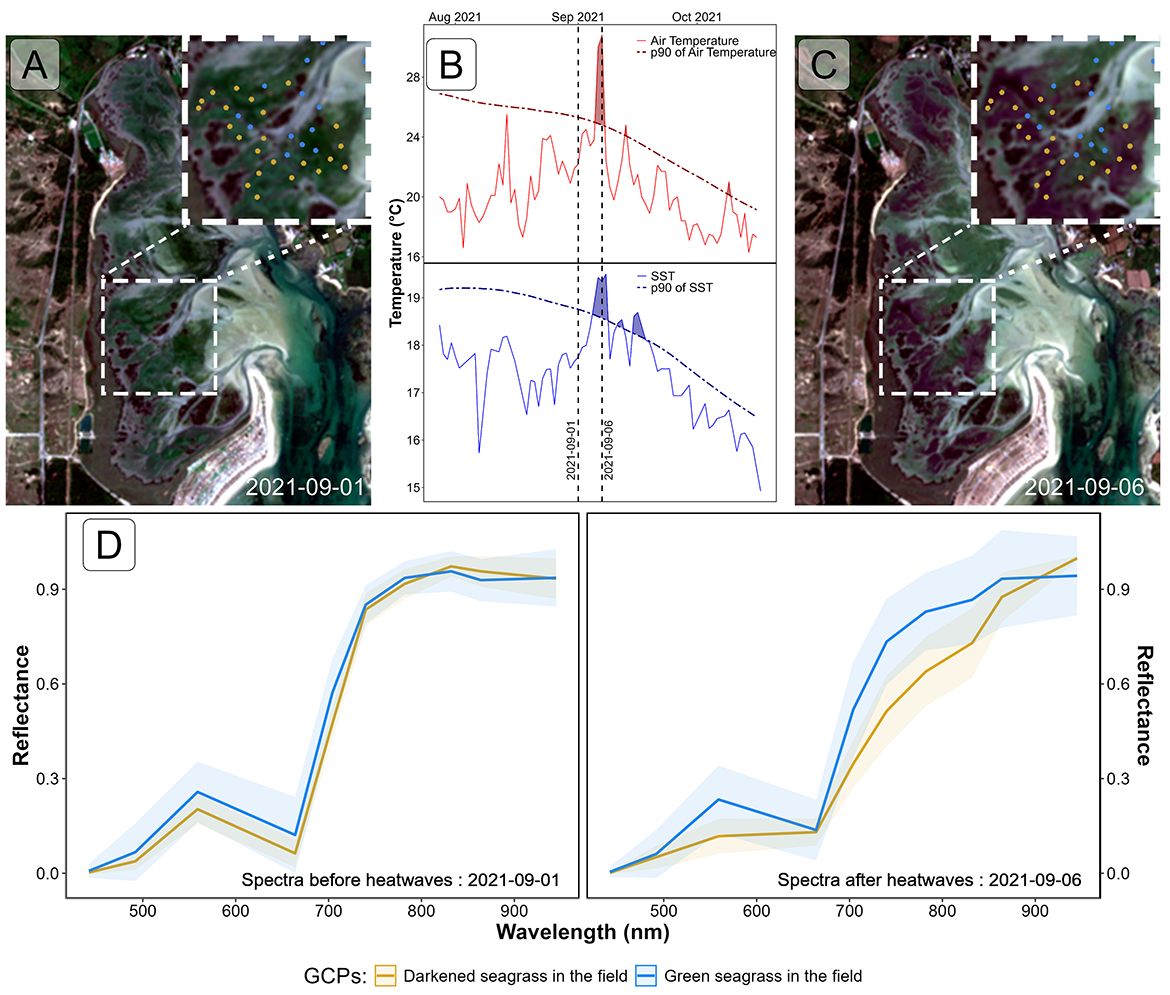
\includegraphics[width=1\textwidth,height=\textheight]{Figs/Low_res/Heatwaves_S2_plot.png}

}

\caption{\label{fig-S2_comparison}Spectral Comparison of Sentinel-2
Reflectance (D) over Ground Control Points (GCPs) Before (A) and During
(B) Heatwave Events (C); A: RGB color composition of the Sentinel-2
image on the 1st of September 2021. The points correspond to GCPs
collected on September 10, 2021 Figure~\ref{fig-quiberonMap}; B:
Detection of heatwave events based on both Air Temperature and Sea
Surface Temperature (SST). The solid line represents the daily average
temperature, while the dashed line indicates the 90th percentile of the
climatology. Colored polygons identidy heatwaves (marine in blue and
atmospherical in red). The two vertical dashed lines represent the
acquisition dates of the two Sentinel-2 images used in this analysis ; C
: RGB color composition of the Sentinel-2 image on the 6th of September
2021. The points correspond to GCPs collected on September 10, 2021
Figure~\ref{fig-quiberonMap} ; D : Average spectral signatures of GCPs
where dark and green seagrasses (blue and gold lines, respectively) were
identified during the field survey. The left plot shows the reflectance
of these GCPs before the heatwave impact, while the right plot shows the
spectral signature during the heatwaves. The ribbons around the lines
represent the standard deviation.}

\end{figure}%

\subsubsection{Radiometric indices
comparison}\label{radiometric-indices-comparison}

Using Sentinel-2 data, the spectral indices (NDVI and GLI) and SPC
estimated for pixels unaffected by the heatwave showed no significant
differences before or during the event (Figure~\ref{fig-NDVI_GLI_SPC},
left column) In contrast, seagrass darkened by the heatwave exhibited a
significant decrease in both index values and SPC
(Figure~\ref{fig-NDVI_GLI_SPC}, right column). In this case, the NDVI
dropped by approximately 34\%, from a median of 0.61 to 0.40, while also
becoming more homogeneous (the standard deviation decreased from 0.09 to
0.06) (Figure~\ref{fig-NDVI_GLI_SPC} B). Although the heatwave did not
affect the observed seagrass density in the field, the drop in NDVI led
to an underestimation of satellite-based SPC, from 83 to 48\%
(Figure~\ref{fig-NDVI_GLI_SPC} D). The GLI, the index that reflects the
greenness of leaves, was the most affected by the event, with an
important reduction from a median of 0.15 to 0.02 during the event
(Figure~\ref{fig-NDVI_GLI_SPC} F). Interestingly, when comparing the
initial seagrass density of both targets (i.e., seagrass density before
the event) pixels affected by the heatwave (median SPC = 65\%;
{[}Figure~\ref{fig-NDVI_GLI_SPC} C green) were denser than the those
remained unchanged (median SPC = 85\%; {[}Figure~\ref{fig-NDVI_GLI_SPC}
D green).

\phantomsection\label{cell-fig-NDVI_GLI_SPC}
\begin{figure}[H]

\centering{

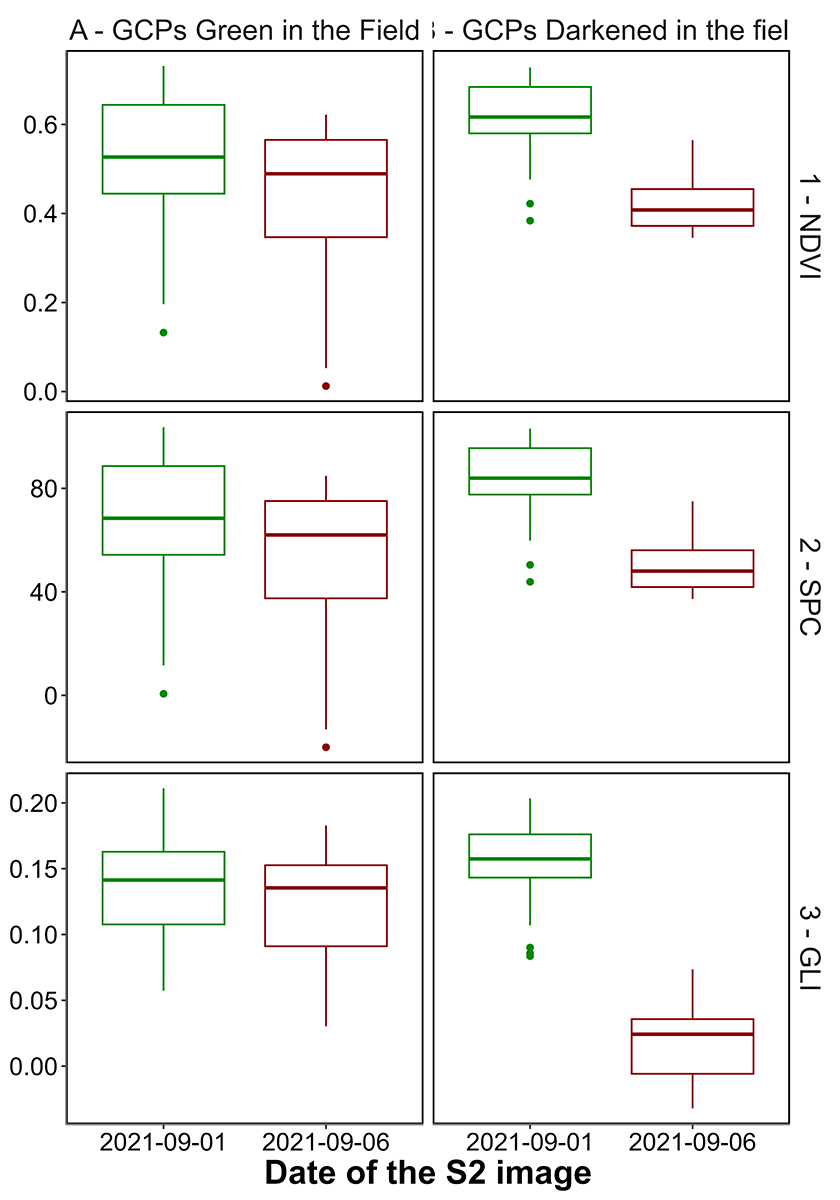
\includegraphics[width=0.8\textwidth,height=\textheight]{Figs/Low_res/Compares_Indices_S2.png}

}

\caption{\label{fig-NDVI_GLI_SPC}Comparaison of Sentinel-2 based
radiometric indices at two different dates, before (2021-09-01, green)
and after (2021-09-06, red) the heatwaves events of Quiberons, for the
two category of GCPs seen in the filed : Green seagrasses (i.e seagrass
not affected by the event, Left Column) and Darkened Seagrasses (i.e
seagrass affected by the event, Right column). The Normalised Difference
Vegetation Index (NDVI) has been computed using the
Equation~\ref{eq-ndvi}, the Seagrass Percent Cover (SPC) with the
Equation~\ref{eq-spc} and the Green Leaf Index (GLI) using
Equation~\ref{eq-gli},}

\end{figure}%

\phantomsection\label{cell-fig-Map_darkening_Bathy}
\begin{figure}[H]

\centering{

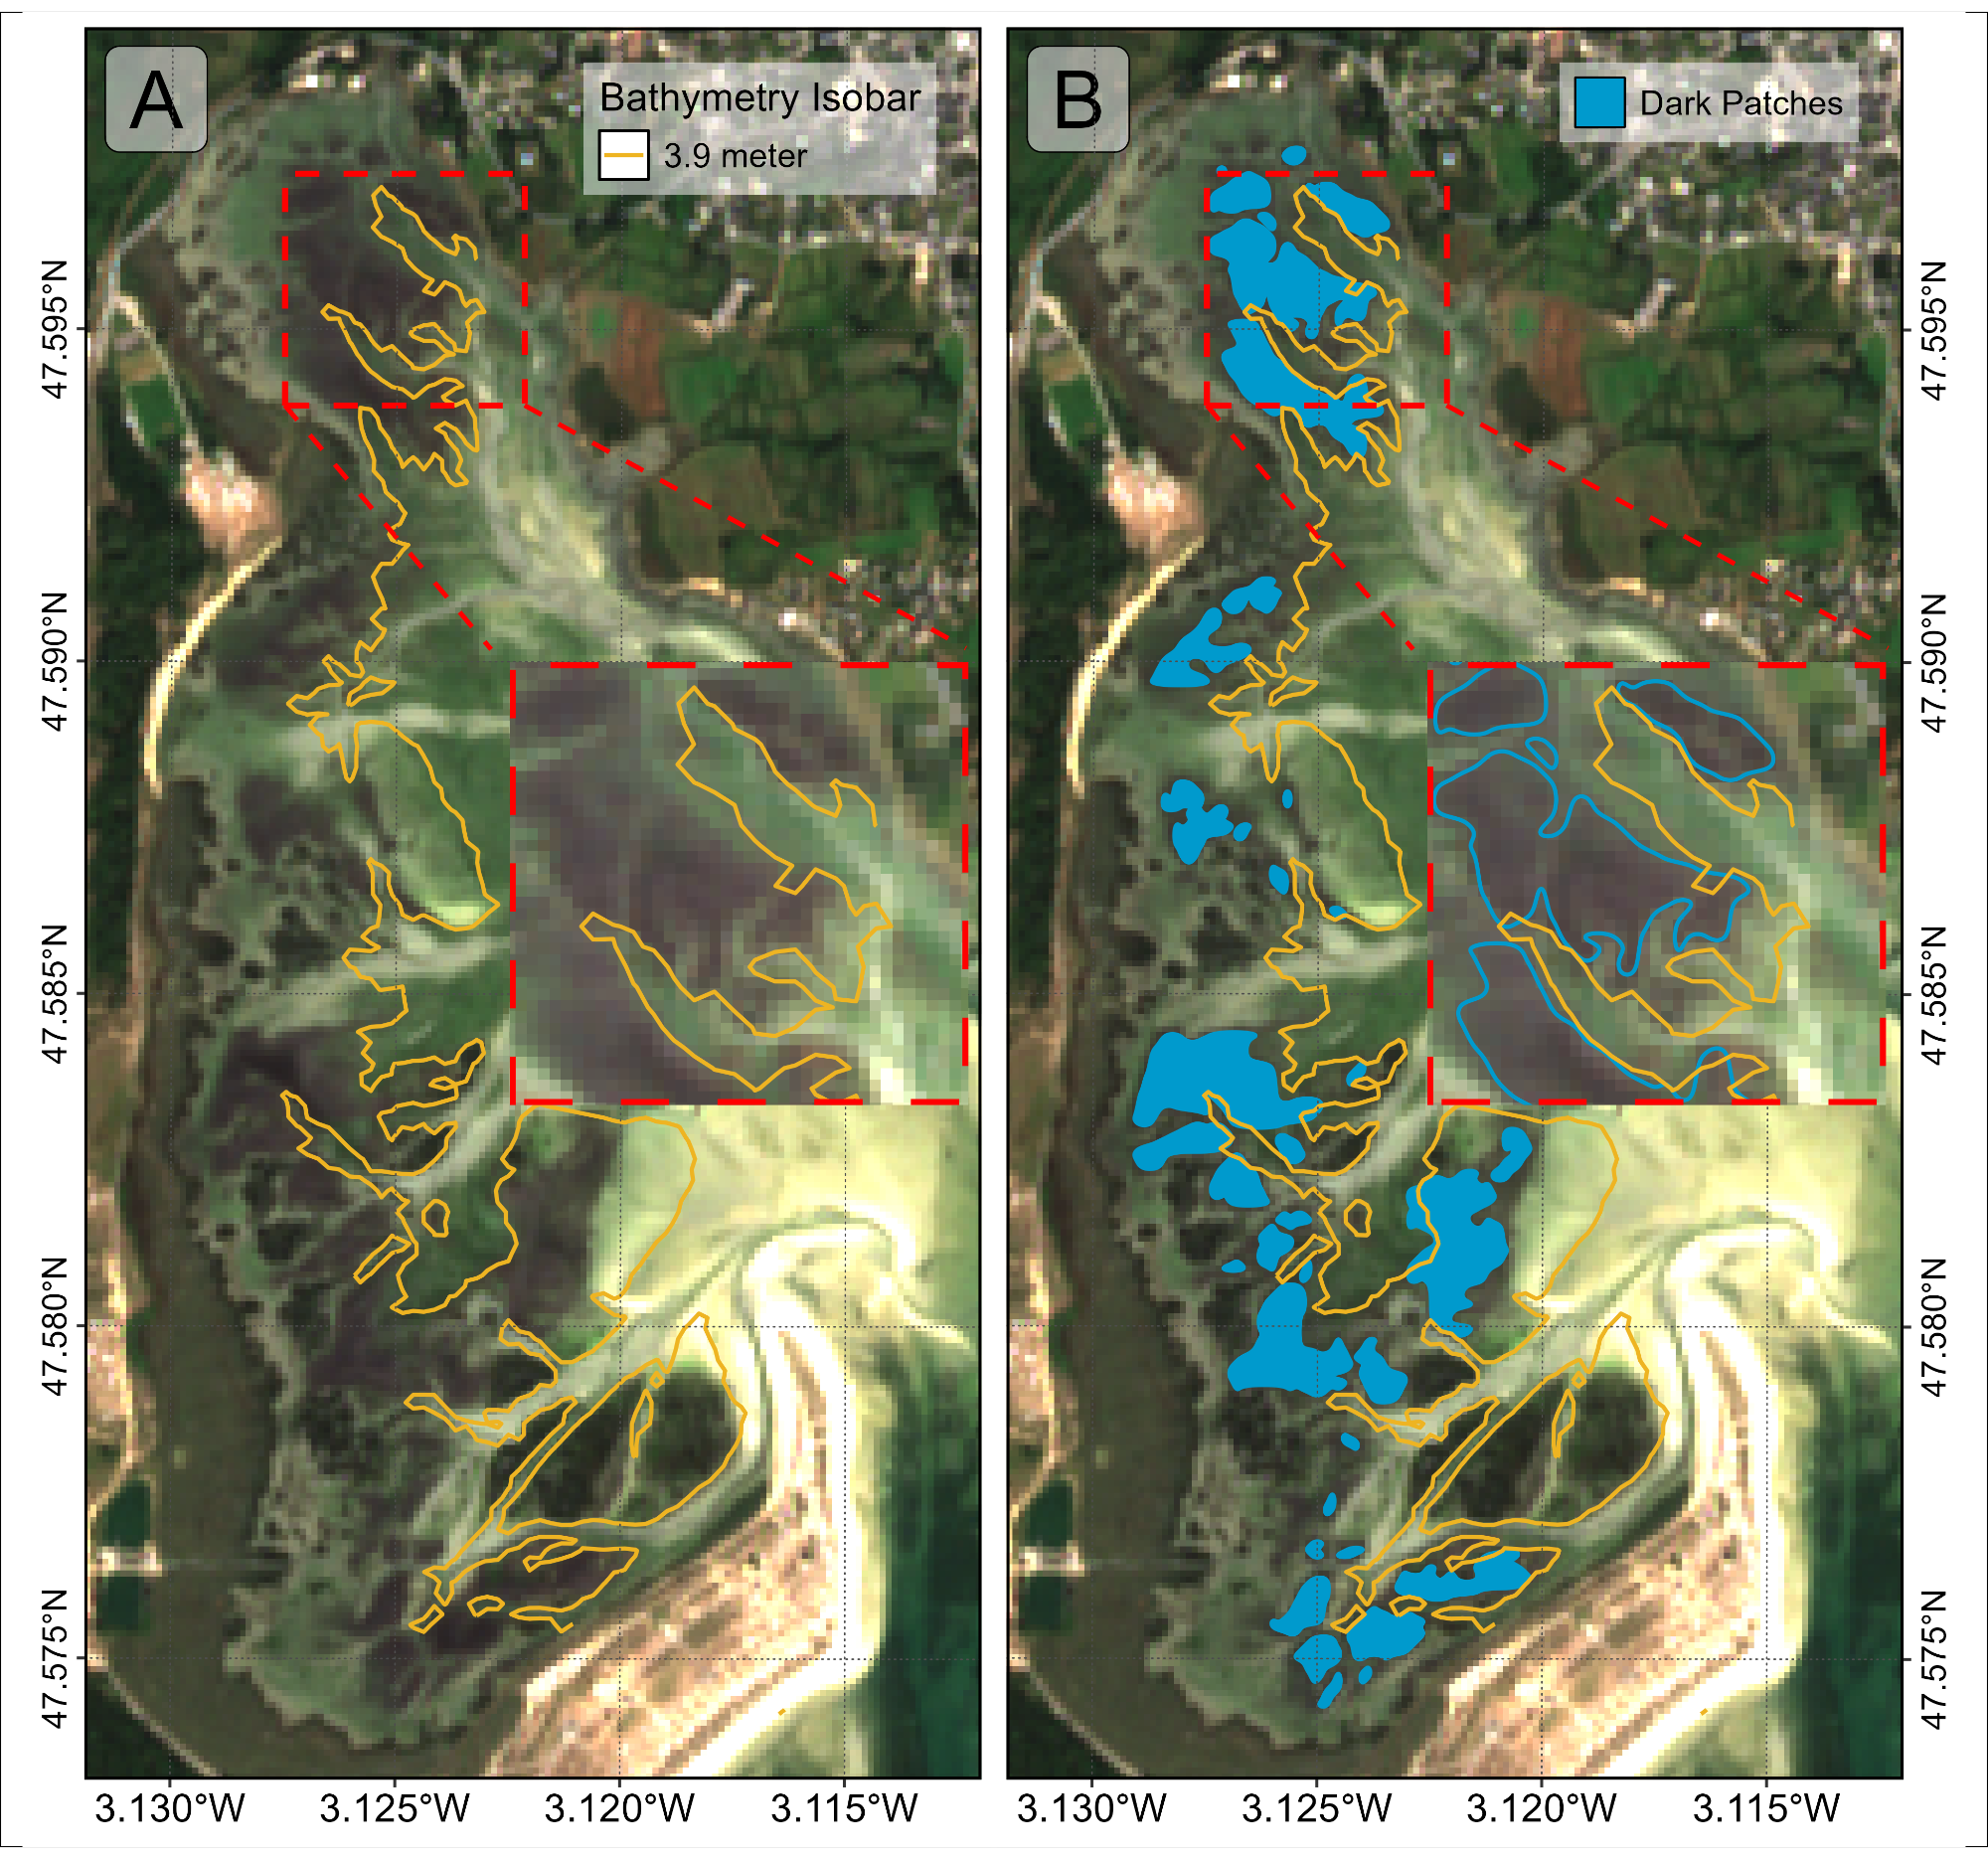
\includegraphics[width=1\textwidth,height=\textheight]{Figs/Low_res/Map_darkening_Bathy.png}

}

\caption{\label{fig-Map_darkening_Bathy}Map of the Darkening of
seagrasses during the heatwave events of September 2021 in Quiberon. A:
1m bathymetry isobar (golden line); B: Result of the detection of
darkened seagrass patches (Blue plolygons)}

\end{figure}%


\renewcommand\refname{Bibliography}
  \bibliography{library.bib}



\end{document}
